% The unit square [0,1]^2 covered by four overlapping epsilon-neighborhoods
% (dotted circles of radius 1/2 centered near the four quadrant directions).
% Source: book/tex/topology/metric-prop.tex (§ Totally bounded spaces) and
%         book/tex/topology/compactness.tex (§ finite subcover example).
\documentclass[border=2mm]{standalone}
\usepackage{tikz}
\begin{document}
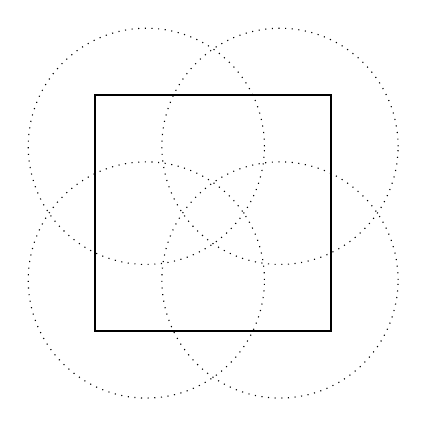
\begin{tikzpicture}[scale=3]
  \draw[black, line width=0.8pt] (-0.5,-0.5) rectangle (0.5,0.5);
  \foreach \a in {45,135,225,315}{
    \draw[dotted] ({0.4*cos(\a)},{0.4*sin(\a)}) circle (0.5);
  }
\end{tikzpicture}
\end{document}
